\section{Eksperymenty i wyniki}

\begin{frame}{Środowiska testowe}
\textbf{Parametry wspólne:}
\begin{itemize}
    \item Polityka próbkowania: $\nu$ -- rozkład jednostajny (eksploracja)
    \item Kroki uczenia: $\eta_n = \frac{\eta_0}{(c + n)^{\kappa}}$, $\theta_n = \frac{\theta_0}{(c + n)^{\lambda}}$ gdzie $\frac{1}{2} < \kappa < \lambda \le 1$
\end{itemize}

\vspace{0.5em}
\textbf{Trzy środowiska testowe:}
\begin{enumerate}
    \item \textbf{MDP z dwoma stanami}
    \begin{itemize}
        \item Prosty model do weryfikacji analitycznej
        \item 2 stany, 2 akcje
        \item Możliwość dokładnego obliczenia wartości teoretycznych
    \end{itemize}
    
    \vspace{0.3em}
    \item \textbf{Problem zarządzania zapasami}
    \begin{itemize}
        \item Dyskretny magazyn o pojemności $M=3$
        \item Losowy popyt, koszty magazynowania i zamówienia
        \item Test algorytmów w realistycznym scenariuszu biznesowym
    \end{itemize}
    
    \vspace{0.3em}
    \item \textbf{Problem przetrwania rozbitka}
    \begin{itemize}
        \item Złożony model zarządzania zasobami
        \item 11~616 stanów, 28 akcji, dynamika stochastyczna
        \item Test skalowalności w dużych przestrzeniach
    \end{itemize}
\end{enumerate}
\end{frame}

\begin{frame}{MDP z dwoma stanami -- Model}
\begin{columns}[T]
\begin{column}{0.48\textwidth}
\textbf{Parametry:}
\begin{itemize}
    \item Stany: $S = \{1, 2\}$
    \item Akcje: $A = \{a_1, a_2\}$
    \item $\alpha = 0.5$, $\beta = 0.9$
\end{itemize}

\vspace{0.3em}
\textbf{Nagrody:}
\begin{itemize}
    \item $r(1,a_1) = 0$, $r(1,a_2) = 2$
    \item $r(2,a_1) = 15$
    \item $r(2,a_2,1) = 20$, $r(2,a_2,2) = 5$
\end{itemize}

\vspace{0.3em}
\textbf{Testowane polityki:}
\begin{itemize}
    \item 4 deterministyczne
    \item 1 mieszana (50/50)
\end{itemize}
\end{column}

\begin{column}{0.48\textwidth}
\centering
\includegraphics[width=0.95\textwidth]{../../thesis/fig/example1.png}
\small Diagram przejść w modelu dwustanowym
\end{column}
\end{columns}
\end{frame}

\begin{frame}{MDP z dwoma stanami -- Wyniki Algorytmu 1}
\textbf{Algorytm ewaluacji polityki -- porównanie z wartościami teoretycznymi:}

\begin{table}[h!]
\centering
\small
\begin{tabular}{lccc}
\toprule
\textbf{Polityka} & \textbf{Stan} & \textbf{$J$ (teoria)} & \textbf{$J$ (aproks.)} \\
\midrule
$\phi_1: (a_1, a_1)$ & 1 & 35.5263 & 35.5175 \\
$\phi_1: (a_1, a_1)$ & 2 & 46.9737 & 46.9643 \\
\midrule
$\phi_3: (a_1, a_2)$ & 1 & 38.7931 & 38.7936 \\
$\phi_3: (a_1, a_2)$ & 2 & 49.3534 & 49.3612 \\
\bottomrule
\end{tabular}
\end{table}

\vspace{0.3em}
\textbf{Obserwacje:}
\begin{itemize}
    \item Błąd aproksymacji < 1\%
    \item Szybka zbieżność (1 000 000 iteracji)
    \item Potwierdzenie poprawności implementacji
\end{itemize}
\end{frame}

\begin{frame}{MDP z dwoma stanami -- Wyniki Algorytmu 2}
\textbf{Uczenie optymalnej polityki (25 000 000 iteracji):}

\begin{table}[h!]
\centering
\small
\begin{tabular}{lrr|rr}
\toprule
\textbf{Stan} & $Q(s,a_1)$ & $Q(s,a_2)$ & $W(s,a_1)$ & $W(s,a_2)$ \\
\midrule
1 & 38.7921 & \textbf{38.8527} & \textbf{77.5813} & 75.6954 \\
2 & \textbf{49.9129} & 49.3519 & 84.8224 & \textbf{86.1988} \\
\bottomrule
\end{tabular}
\end{table}

\vspace{0.3em}
\textbf{Optymalne polityki:}
\begin{itemize}
    \item $\mu^\star$: $\{1: a_2, 2: a_1\}$ -- impulsywna (pierwszy krok)
    \item $\phi_s^\star$: $\{1: a_1, 2: a_2\}$ -- planowa (kontynuacja)
\end{itemize}

\vspace{0.3em}
\textbf{Kluczowa obserwacja:}
\begin{itemize}
    \item \textbf{Niespójność czasowa:} $\mu^\star \neq \phi_s^\star$ dla $\alpha < 1$
    \item Decydent zobowiązany osiąga lepsze wyniki niż naiwny
\end{itemize}
\end{frame}

\begin{frame}{Problem zarządzania zapasami}
\textbf{Model:}
\begin{itemize}
    \item Pojemność magazynu: $M = 3$ (4 stany: 0, 1, 2, 3)
    \item Popyt losowy: $D \in \{0, 1, 2\}$ z rozkładem $(0.2, 0.3, 0.5)$
    \item Koszty: zakup $c=5$, magazynowanie $h=2$, przychód ze sprzedaży $p=9$
    \item Parametry: $\alpha = 0.5$, $\beta = 0.9$
\end{itemize}

\vspace{0.5em}
\textbf{Testowane pary polityk:}
\begin{itemize}
    \item $\rho_1 = (\mu^\star, \phi_s^\star)$ -- optymalne (z Algorytmu 2)
    \item $\rho_2 = (\nu, \phi_s^\star)$ -- jednostajny pierwszy krok
    \item $\rho_3 = (\mu^\star, \nu)$ -- jednostajna kontynuacja
\end{itemize}

\vspace{0.5em}
\textbf{Wyniki (5 000 000 iteracji):}
\begin{itemize}
    \item Wszystkie aproksymacje zbiegły do wartości teoretycznych
    \item $\rho_1$ osiąga najwyższe wartości we wszystkich stanach
    \item Potwierdzenie skuteczności obu algorytmów
\end{itemize}
\end{frame}

\begin{frame}{Problem zarządzania zapasami -- Zbieżność}
\begin{figure}[htbp]
    \centering
    
\includegraphics[width=0.8\textwidth]{../../data/plots/ex2Plots.png}
    \caption{Zbieżność błędu normy $\ell_2$ aproksymacji $W$ i $J$ dla trzech par polityk (skala logarytmiczna)}
\end{figure}

\textbf{Obserwacje:}
\begin{itemize}
    \item Wykładnicza zbieżność zgodna z teorią
    \item Para $\rho_1$ zbiega najszybciej (optymalna polityka próbkowania)
\end{itemize}
\end{frame}

\begin{frame}{Problem przetrwania rozbitka -- Model}
\textbf{Założenia:}
\begin{itemize}
    \item Rozbitek na bezludnej wyspie zarządza zasobami (jedzenie, woda, zdrowie)
    \item Stan: $(f, w, h, d)$ -- jedzenie (0--10), woda (0--10), zdrowie (0--5), dni (0--15)
    \item Przestrzeń stanów: $11 \times 11 \times 6 \times 16 = 11\,616$ stanów
    \item Limit czasu: 15 dni (potem wyspa zalewa się)
\end{itemize}

\vspace{0.3em}
\textbf{Akcje (28 kombinacji):}
\begin{itemize}
    \item Tryb: czekaj, połów, ekspedycja ratunkowa
    \item Konsumpcja jedzenia: 0, 1 lub 2 jednostki
    \item Konsumpcja wody: 0, 1 lub 2 jednostki
\end{itemize}

\vspace{0.3em}
\textbf{Dynamika:}
\begin{itemize}
    \item Pogoda: deszcz z prawd. 50\% (+2 lub +3 wody)
    \item Połów: wymaga 1 jedz.+1 wody, daje 3 jedzenia (szansa rośnie ze zdrowiem)
    \item Ekspedycja: wymaga 7 jedz.+7 wody oraz $h \geq 3$, szansa zależy od zdrowia i zapasów
    \item Ratunek losowy: 7\% dziennie od dnia 2
\end{itemize}
\end{frame}

\begin{frame}{Problem przetrwania rozbitka -- Wyniki}
\textbf{Symulacja Monte Carlo (500 000 prób):}

\begin{table}[h!]
\centering
\begin{tabular}{lr}
\toprule
\textbf{Polityka} & \textbf{Wskaźnik przeżycia [\%]} \\
\midrule
Impulsywna ($\mu^\star$) & 41.85 \\
Planowa ($\phi_s^\star$) & 43.26 \\
Mieszana ($\mu^\star, \phi_s^\star$) & 43.19 \\
Losowa (jednostajna) & 12.81 \\
Człowiek (50 prób) & 42.00 \\
\bottomrule
\end{tabular}
\end{table}

\vspace{0.3em}
\textbf{Obserwacje:}
\begin{itemize}
    \item Algorytmy osiągają wyniki porównywalne z człowiekiem
    \item Polityka planowa ($\phi_s^\star$) nieznacznie lepsza od impulsywnej
    \item Polityka losowa dramatycznie gorsza ($\sim$3x niższa przeżywalność)
    \item Główna różnica: strategia podejmowania ekspedycji w dniu 4
\end{itemize}
\end{frame}

\begin{frame}{Problem przetrwania rozbitka -- Analiza}
\begin{columns}[T]
\begin{column}{0.48\textwidth}
\centering

\includegraphics[width=0.95\textwidth]{../../data/plots/distributioncastaway.png}
\small Rozkład zgonów i ratunków
\end{column}
\begin{column}{0.48\textwidth}
\centering

\includegraphics[width=0.95\textwidth]{../../data/plots/expeditions.png}
\small Rozkład wypraw ratunkowych
\end{column}
\end{columns}

\vspace{0.3em}
\textbf{Kluczowe wnioski:}
\begin{itemize}
    \item Polityki $\phi_s^\star$ i $(\mu^\star, \phi_s^\star)$ podejmują ekspedycje w dniu 4
    \item To pozwala utrzymać wysoki poziom ratunków z dnia 3
    \item Nagroda za przetrwanie przeważa nad pokusą natychmiastowej konsumpcji
    \item Model QH dobrze oddaje trade-off między krótko- i długoterminowymi celami
\end{itemize}
\end{frame}

\begin{frame}{MDP z dwoma stanami -- Model}
\begin{columns}
\begin{column}{0.5\textwidth}
\textbf{Definicja modelu:}
\begin{itemize}
    \item Stany: $S = \{1, 2\}$
    \item Akcje: $A = \{a_1, a_2\}$
    \item Parametry: $\alpha = 0.5$, $\beta = 0.9$
\end{itemize}

\vspace{0.5em}
\textbf{Nagrody:}
\begin{itemize}
    \item $r(1,a_1) = 0$
    \item $r(1,a_2) = 2$
    \item $r(2,a_1) = 15$
    \item $r(2,a_2) = 20$ lub $5$
\end{itemize}

\vspace{0.5em}
\textbf{Testowane polityki:}
\begin{itemize}
    \item 4 deterministyczne
    \item 1 mieszana (50/50)
\end{itemize}
\end{column}

\begin{column}{0.5\textwidth}
\begin{figure}
    \centering
    \includegraphics[width=\textwidth]{../thesis/fig/example1.png}
    \caption*{Diagram przejść w modelu dwustanowym}
\end{figure}
\end{column}
\end{columns}
\end{frame}

\begin{frame}{MDP z dwoma stanami -- Wyniki}
\textbf{Weryfikacja poprawności algorytmów:}

\begin{itemize}
    \item Porównanie wyników z obliczeniami analitycznymi
    \item Algorytmy osiągnęły zbieżność do wartości teoretycznych
    \item Błąd aproksymacji poniżej 1\%
\end{itemize}

\vspace{0.5em}
\textbf{Obserwacje:}
\begin{itemize}
    \item \textbf{Niespójność czasowa:} Optymalna reguła pierwszego kroku $\mu^\star$ różni się od optymalnej polityki stacjonarnej $\phi_s^\star$ dla $\alpha < 1$
    \item Decydent zobowiązany osiąga wyższą wartość niż decydent naiwny
    \item Szybka zbieżność (wykładnicza) zgodnie z teorią
\end{itemize}

\vspace{0.5em}
\textbf{Warunki Robbinsa-Monro dla kroków uczenia:}
\[
\eta_n = \frac{\eta_0}{(c + n)^{\kappa}}, \quad
\theta_n = \frac{\theta_0}{(c + n)^{\lambda}}, \quad
\frac{1}{2} < \kappa < \lambda \le 1
\]
\end{frame}

\begin{frame}{Problem zarządzania zapasami}
\textbf{Model:}
\begin{itemize}
    \item Decydent zarządza magazynem z ograniczoną pojemnością
    \item W każdym okresie podejmuje decyzję o zamówieniu
    \item Popyt jest losowy
    \item Koszty: przechowywania, zamówienia, braku zapasu
\end{itemize}

\vspace{0.5em}
\textbf{Parametry środowiska:}
\begin{itemize}
    \item Maksymalna pojemność magazynu: różne konfiguracje
    \item Rozkład popytu: dyskretny, losowy
    \item Dyskontowanie QH: $\alpha = 0.5$, $\beta = 0.9$
\end{itemize}

\vspace{0.5em}
\textbf{Cele eksperymentu:}
\begin{enumerate}
    \item Weryfikacja działania algorytmu w bardziej złożonym środowisku
    \item Analiza zachowania decydenta z uprzedzeniem teraźniejszości
    \item Porównanie z klasycznym podejściem wykładniczym ($\alpha = 1$)
\end{enumerate}
\end{frame}

\begin{frame}{Problem przetrwania rozbitka -- Model}
\textbf{Założenia:}
\begin{itemize}
    \item Rozbitek na bezludnej wyspie musi zarządzać zasobami (jedzenie, woda)
    \item Stan: $(f, w, h, d)$ -- jedzenie, woda, zdrowie, dni na wyspie
    \item Przestrzeń stanów: $11 \times 11 \times 6 \times 16 = 11\,616$ stanów
    \item Limit czasu: maksymalnie 15 dni (potem wyspa zalewa się)
\end{itemize}

\vspace{0.5em}
\textbf{Akcje (28 kombinacji):}
\begin{itemize}
    \item Tryb: \textit{czekaj}, \textit{połów}, \textit{ekspedycja ratunkowa}
    \item Konsumpcja jedzenia: 0, 1 lub 2 jednostki
    \item Konsumpcja wody: 0, 1 lub 2 jednostki
\end{itemize}

\vspace{0.5em}
\textbf{Dynamika:}
\begin{itemize}
    \item Pogoda: deszcz z prawd. 50\% (+2 lub +3 wody)
    \item Połów: wymaga 1 jedz.+1 wody, daje 3 jedzenia (szansa rośnie ze zdrowiem)
    \item Ekspedycja: wymaga 7 jedz.+7 wody i $h \ge 3$ (może zakończyć epizod ratunkiem)
\end{itemize}
\end{frame}

\begin{frame}{Problem przetrwania rozbitka -- Dynamika i nagrody}
\textbf{Mechanika zdrowia:}
\begin{itemize}
    \item Zmiana zdrowia zależy od konsumpcji:
    \begin{itemize}
        \item $+1$ przy jedzeniu i wodzie $\ge 2$ jednostki każdego
        \item $0$ przy jedzeniu i wodzie $\ge 1$ jednostki każdego
        \item $-1$ w pozostałych przypadkach
        \item $-2$ przy braku jedzenia i wody
    \end{itemize}
    \item Szansa przeżycia nocy: 0.0 (h=0), 0.5 (h=1), 0.75 (h=2), 0.9 (h=3), 0.95 (h=4), 0.99 (h=5)
    \item Ratunek losowy: 7\% dziennie od drugiego dnia
\end{itemize}

\vspace{0.5em}
\textbf{Funkcja nagrody:}
\[
r(s,a,s') = \left[\log(1 + c^f) + \log(1 + c^w)\right] \cdot \left(1 + \left(\frac{h'}{H_{\max}}\right)^2\right) + r_{\text{term}}
\]
gdzie $r_{\text{term}} = +50$ (ratunek), $-100$ (śmierć), $0$ (w trakcie gry)

\vspace{0.5em}
\textbf{Parametry QH:} $\alpha = 0.6$, $\beta = 0.95$
\end{frame}

\begin{frame}{Problem przetrwania rozbitka -- Wyniki}
\textbf{Wskaźniki przeżycia (Monte Carlo, 500~000 symulacji):}

\vspace{0.3em}
\begin{table}[h!]
\centering
\begin{tabular}{l r}
\toprule
Polityka & Przeżywalność [\%] \\
\midrule
Impulsywna ($\mu^\star$) & 41.85 \\
Planowa ($\phi^\star$) & 43.26 \\
Mieszana ($\mu^\star, \phi^\star$) & 43.19 \\
Losowa (jednostajna) & 12.81 \\
Sterowanie manualne (autor) & 42.00 \\
\bottomrule
\end{tabular}
\end{table}

\vspace{0.5em}
\textbf{Obserwacje:}
\begin{itemize}
    \item Nawet agent impulsywny osiąga wysoką przeżywalność
    \item Główna różnica: timing ekspedycji ratunkowych
    \item Polityki $\phi^\star$ i mieszana podejmują ekspedycje wcześniej (dzień 4)
    \item Polityka losowa: drastycznie niższa przeżywalność
\end{itemize}
\end{frame}

\begin{frame}{Wyniki eksperymentów -- Zarządzanie zapasami}
\textbf{Kluczowe obserwacje:}

\begin{itemize}
    \item \textbf{Różnica w strategiach:} Decydent QH ($\alpha < 1$) preferuje natychmiastowe nagrody
    \begin{itemize}
        \item Mniejsze zamówienia w pierwszym kroku
        \item Wyższa gotowość akceptacji kosztów braku zapasu
    \end{itemize}
    
    \vspace{0.5em}
    \item \textbf{Zbieżność:} Algorytm QH Q-Learning skutecznie nauczył się polityki
    \begin{itemize}
        \item Stabilizacja wartości Q po odpowiedniej liczbie iteracji
        \item Zgodność z przewidywaniami teoretycznymi
    \end{itemize}
    
    \vspace{0.5em}
    \item \textbf{Porównanie z decydentem wykładniczym:}
    \begin{itemize}
        \item Decydent wykładniczy ($\alpha = 1$) osiąga wyższe wartości długoterminowe
        \item Decydent QH ($\alpha < 1$) maksymalizuje wartość uwzględniając uprzedzenie teraźniejszości
        \item Różne strategie optymalne dla różnych wartości $\alpha$
    \end{itemize}
\end{itemize}
\end{frame}

\begin{frame}{Implementacja i metodologia}
\textbf{Narzędzia i technologie:}
\begin{itemize}
    \item Język: Python 3.8+
    \item Biblioteki: NumPy, SciPy, Matplotlib
    \item Framework testowy: pytest
\end{itemize}

\vspace{0.5em}
\textbf{Struktura kodu:}
\begin{itemize}
    \item \texttt{algorithms/} -- implementacje algorytmów (QH Q-Learning, Policy Evaluation)
    \item \texttt{models/} -- modele środowisk (Inventory, GridWorld)
    \item \texttt{experiments/} -- framework eksperymentalny
    \item \texttt{tests/} -- testy jednostkowe
\end{itemize}

\vspace{0.5em}
\textbf{Walidacja:}
\begin{itemize}
    \item Porównanie z wynikami analitycznymi dla prostych modeli
    \item Testy zbieżności
    \item Weryfikacja własności teoretycznych (kontrakcja, niespójność czasowa)
\end{itemize}
\end{frame}
